\chapter{Design requirements and architectural choices}
\label{ch:design}

This chapter will discuss multiple architectural design choices to build a Reference Model. This chapter will focus on the overall design and architecture, while \Cref{ch:PipelineShell} and \Cref{ch:ISS} will focus on the details of the pipeline shell and ISS. Each of these chapters will feature a requirement list for the components. Throughout the chapter, requirements for ISS will be indicated with \textbf{ISS requirement X}, and requirements for the pipeline shell will be indicated with \textbf{PS requirement X}, both linking to the corresponding requirements at the beginning of each corresponding chapter.

\section{Reference Model Requirements}
\tmp{TODO}
The main challenges discussed in \cref{sec:back_issProblem} are that when using an ISS as a reference model, asynchronous events can be taken at the wrong time or in the wrong order, and the timing of the side effects can vary between the DUT and the reference model. This happens because the ISS does not have the necessary core-specific pipeline understanding to know how to respond to these asynchronous events.

To overcome these challenges, we should build a reference model that adds a pipeline understanding to the model and use this to time asynchronous events and side effects correctly.

Since testbenches shared by multiple cores, like core-v-verif, have become more common, the effort required to modify the reference model for a new core should be as low as possible.



%In \cref{sec:architecture}, we will discuss the basic architecture of the model, partitioning the design into a pipeline shell and an ISS. \Cref{sec:inOut} will cover the inputs and outputs to the model, \cref{sec:shell_iss_interaction} will discuss the different options for the interaction and partitioning of the model into the pipeline shell and the ISS. \Cref{sec:pipelineShell} will cover the implementation choices for the pipeline shell, and \cref{sec:choosingISS} will compare different Instruction Set Simulators to use in the reference model.

The requirements of the reference model are collected in the requirement list below to concretize the model's development.


\begin{enumerate}
    \item \textbf{The order of the retired instructions should exactly match the core.} \label[rmReq]{rmReq:order}
    \par This requirement expresses the main problem the reference model should solve, avoiding problems like the example shown in \Cref{fig:lw_example}. Note that the requirement does not specify full cycle-accurate simulation; only accurate timing of instructions is required. Although cycle-accurate modeling might be required to order instructions correctly with asynchronous events, this also opens up the possibility of other approaches.
    
    \item \textbf{The reference model should not allow more state changes than the core } \label[rmReq]{rmReq:}
    \par This requirement highlights the problem with ImperasDV described in \ref{}.

    \item \textbf{Read the same ELF binary file as the core} \label[rmReq]{rmReq:binary}
    \par The reference model must be able to run the same test program as the core, requiring that it can run the same ELF binary file as the core without any modifications to the program or memory map.

    \item \textbf{Output the state changes for comparison at every instruction retirement} \label[rmReq]{rmReq:stateOutput}
    \par To be able to compare the execution of the reference model with the core, we must output the state changes at every instruction retirement. Since the cores in core-v-verif support \acrshort{rvfi} \cite{}, we should also output the state changes as \acrshort{rvfi} or the superset \acrshort{rvvi}.

    \item \textbf{Take interrupts and debug requests as inputs independently of the core.} \label[rmReq]{rmReq:asyncInputs}
    \par As described in \ref{}, an ISS can take asynchronous events in sync with the core by not taking these events directly as inputs but instead using the \acrshort{rvfi} output from the core to take the same interrupt or debug request as the core. With the reference model, we want to avoid the verification hole that occurs when the ISS only follows asynchronous events of the core and does not actually decide for itself which event to take. 

    \item \textbf{Configurable with the same extensions supported by the core.} \label[rmReq]{rmReq:extensions}
    \par Some cores allow for different extensions to be enabled or disabled. In order to match the core, the reference model should also be configurable with different RISC-V extensions.\textbf{\Cref{issReq:custom}}
    
    \item \textbf{The RM should be as easy as possible to modify to support different cores.} \label[rmReq]{rmReq:modifyable}
    \par The reference model should be usable by different cores, so the effort required to adapt the reference model to a new core should be as low as possible.
    
   % \item \textbf{Run in lock-step with the core} \label[rmReq]{rmReq:lock-step}
   % \par 
   
   % \item \textbf{Run in the core-v-verif UVM verification environment} \label[rmReq]{rmReq:core-v-verif}
   % \par 

    \item \textbf{Avoid prohibiting support for formal verification} \label[rmReq]{rmReq:formal}
    \par If possible, the reference model should be able to support formal verification. At every design choice, formal verification should be kept in mind.
    
    
\end{enumerate}

\Cref{rmReq:order}


\section{Architecture}
\tmp{TODO: Må utdypes endel}

As discussed in \Cref{sec:pw_architecture}, the specialization report proposed implementing the reference model with a two-layered modeling technique inspired by the work of \textcite{chiangEfficientTwolayeredCycleaccurate2009} and \textcite{leeFaCSimFastCycleAccurate2008}, which both divided the model into one untimed functional simulator and one timing shell responsible for correctly timing the results generated in the functional simulator. This way, the functional simulator can be general enough to be used by many different cores, while all the core-specific functionality is contained in the timing shell.

In order to fulfill \Cref{rmReq:modifyable}, we implement a similar two-layered division of functionality and timing instead of implementing or modifying a full microarchitectural simulator like gem5 \cite{Gem5Simulator2023} that combines both. This makes configuring the reference model to a new core easier since all the core-specific details should be contained together. 

As discussed in \Cref{sec:pw_architecture}, we can use an existing \acrshort{iss} as the functional simulator and implement the core-specific timing module around it, which we will call the \gls{ps} from now on. An ISS steps one instruction at a time and completely finishes all execution of an instruction before moving on to the next. This makes it easy to export a \ccode{step()} function that allows the ISS to do an untimed step, executing one instruction at a time. Since the ISS contains all the functionality, including registers and memory, it must also return the state changes caused by the instruction. This can then be passed to the pipeline shell to time these changes correctly and use them to control the ISS.


\Cref{fig:architecture} shows a block diagram of the proposed architecture for the reference model and relevant surrounding modules.\tmp{explain figure}

\tmp{How is core specific funtionality is kept separate}



\begin{figure}
    \centering
    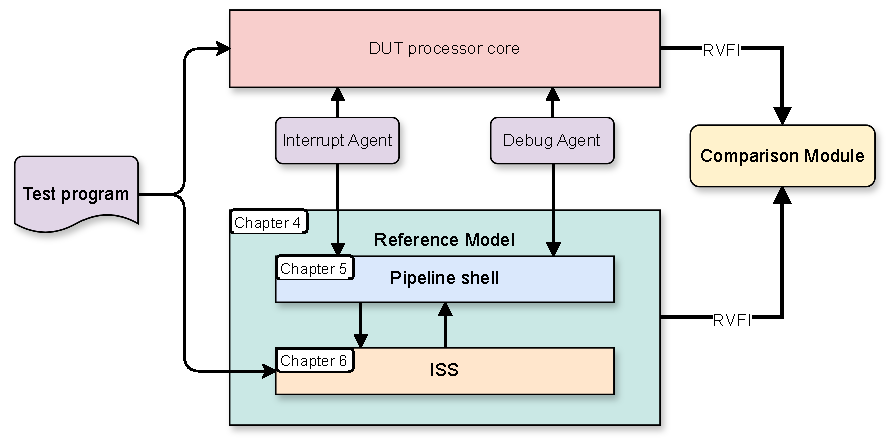
\includegraphics[width=0.75\linewidth]{figures/Architecture.pdf}
    \caption{Block diagram of the reference model architecture.}
    \label{fig:architecture}
\end{figure}

\section{Reference Model language}

The core-v-verif is mainly written in SystemVerilog \cite{openhwgroupOpenhwgroupCorevverif2023}, while many ISSs are written in C++ or other high-level languages \cite{SpikeRISCVISA2023}.
We therefore have to decide what language to implement the reference model in.

In order to fulfill \textbf{\Cref{rmReq:formal}} and have the possibility of using formal verification, it is best to model the simulator in SystemVerilog. This also makes it easier to pass in nets from the rest of the testbench and model parallel components like the pipeline. One disadvantage of using the same language as the core we want to model, is that we are more likely to model the reference model similar to the core, potentially modeling the same bugs in both. 

Considering this disadvantage, we still choose to model as much of the reference model as possible in SystemVerilog. 

\section{Reference Model Interface}
\label{sec:rmInterface}

\subsection{RVVI or custom interface}

We can choose to use RVVI or create our own interface to interface with the reference model and related testbench components. The RVVI-API is a standard set of API calls meant to decouple the testbench from a specific reference model by abstracting away its details \cite{riscv-verificationRISCVVerificationInterface2023}. 

To comply with \Cref{rmReq:formal} we want to avoid limiting the possibility of supporting formal verification where this is possible. RVVI is not implemented with formal verification in mind and has multiple problems regarding formal verification. One example of this is the \sv{net_push()} and \sv{net_pop()} functions used to pass asynchronous net changes to the reference model, which utilize dynamic arrays. Dynamic arrays are not synthesizable in SystemVerilog \cite{mehtaIntroductionSystemVerilog2021} and are, therefore, not compatible with formal verification. 

Additionally the CV32E40S and other OpenHW cores currently support RVFI, but not the RVVI-Tracer. This currently requires converting the RVFI signals to RVVI-Trace signals that are passed to the reference model over the RVVI-API. 
Although RVVI in itself is open, many of the complimentary components like \sv{trace2cov}, \sv{trace2api}, and \sv{trace2log} are proprietary Imperas components. To use RVVI for our reference model, we would have to model replacements for these components anyway it order to convert from RVVI-Trace to RVVI-API. 

The design of RVVI also adds some limitations to how the reference model can be built and still support RVVI. Although RVVI is an open standard, it was developed by Imperas and is influenced by the design of ImperasDV. The RVVI-API supports a step-and-compare methodology, where all controls are based on functions. This includes functions for passing the DUT states to the reference model and functions for comparing each state\cite{riscv-verificationRISCVVerificationInterface2023}. As will be discussed further in \ref{}, we also want to implement a compare module that supports assertions, which is complicated by the design of RVVI. 
In \Cref{sec:ps_dependency}, we will also discuss how the reference model should depend on the core. Here, the design of RVVI implicitly restricts our choices. 

To keep our implementation choices independent of RVVI's design and also keep support for formal verification possible, we choose not to support RVVI during the development of the model. Instead, we will make our own interface that can grow to complement the functionality of the reference model. If we discover that the chosen design is compatible with RVVI, support for this can be added in the future, as there are many advantages to using a standardized interface \cite{riscv-verificationRISCVVerificationInterface2023}.


\subsection{Inputs}

To support formal verification, we want to mainly use normal synthesizable nets as inputs and outputs to the reference model instead of communicating with functions.

\subsubsection{clock and reset}

Compared to ImperasDV, which uses RVVI functions to report reset, retirements, net changes, we want to use normal nets. Because of this we use normal clock and reset signals from the \sv{clknrst_if} clock and reset interface. 

\subsubsection{Binary file}
In order to fulfill \Cref{rmReq:binary}, we must be able to load an ELF binary file. We therefore need some way of inputting the file path of a binary file into the reference model. In core-v-verif, the path to the binary file is loaded through a command line argument. Since the reference model should run the exact same program, we can read this path inside the reference model wrapper, where we can pass it to the reference model.

\subsubsection{Asynchronous events}
In order to fulfill \Cref{rmReq:asyncInputs}, the reference model should have the same asynchronous event inputs as the core. 

Interrupts can be passed to the reference mode from the 32-bit \sv{interrupt_if.irq} signal, and the debug requests are passed through the \sv{debug_if.debug_req} signal.


\subsubsection{Core-dependent inputs}

Depending on the implementation of the pipeline shell, we also want to inform the reference model every time the core retires an instruction. This is reported from the core through \acrshort{rvfi}, via the \sv{rvfi_valid} signal. The use of this signal will be discussed further in \Cref{sec:ps_dependency}.

\subsection{Outputs}

Because the CV32E40S core and other OpenHW cores use RVFI, it makes sense for the reference model also to output RVFI. This makes it easy to compare the state changes between the core and reference model without converting to another trace interface like RVVI-Trace. 

\subsection{Inputs and outputs}

\begin{itemize}
    \item IN: clk
    \item IN: reset
    \item IN: \sv{irq}
    \item IN: \sv{debug_req}
    \item IN: core retirement \sv{rvfi_valid}
    \item OUT: RVFI
\end{itemize}


\section{Partitioning between ISS and Pipeline shell}

The specialization project also discussed different partitionings and the corresponding interaction between the Pipeline Shell and ISS, described in \Cref{sec:pw_partition}. The report discussed 3 different partitionings, and concluded with a partition that keeps the ISS intact, and a \sv{step()} function executes one whole instruction, and returns only the state changes from this instruction. 

We want to fulfill \Cref{rmReq:modifyable} and make the reference model modifiable to different cores. To accomplish this, we should clearly separate core-specific functionality, from core-independent functionality. To adhere to the two-layered approach discussed above, we do not want any core-specific details in the ISS, but we still want the ISS to do most of the functional execution. 

Because of this, and because we want to limit the modifications to the ISS as much as possible, we choose to load the ELF binary file directly into the ISS instead of into the pipeline shell. This gives us \textbf{\Cref{issReq:binaries}}. Additionally, we will use the GPRs, CSRs, PC, and other registers inside the ISS instead of copying them to the pipeline shell. As discussed in \Cref{sec:pw_partition}, using the registers local to the ISS, we also avoid simulating forwarding, since all the modifications from an instruction is completed before the next instruction is started.

Using the same rationale; we also want to use the memory simulator inside the ISS.

One disadvantage of using the local registers and memory of the ISS is that these can contain some core-specific functionality like memory mapping and implementation-specific changes to \acrshort{csr}s. This leads to an ISS that is not fully core-independent. Because many of these details are can be configured once when configuring the ISS, we can allow this. This gives us \textbf{\Cref{issReq:csr}}, stating that the ISS must be configurable to match the core.

Because the ISS is responsible for the functional execution of the instruction, it also needs to be configurable to support different RISC-V extensions, as expressed in \textbf{\Cref{rmReq:extensions}}. This gives us \textbf{\Cref{issReq:custom}}. \tmp{sjekk req.}


Because the ISS is responsible for fetching instructions, executing the instructions, updating registers, and writing to and from memory, this needs to be reported out of the ISS as well. All of this should then be reported out of the ISS and handled and timed by the pipeline shell. We want to use a standard interface to report these changes because we want to support the possibility of exchanging the ISS in the future. Since we want to use RVFI as an output of the reference model, it also makes sense to report state changes from the ISS using RVFI. This gives us \textbf{\Cref{issReq:state}} and \textbf{\Cref{psReq:rvfi}}.

\section{ISS Interface}

\tmp{Move to \Cref{ch:ISS}}?

\tmp{Rewrite:}

\begin{itemize}
    \item Use a wrapper to easily change out ISS later
    \item Use functions to interface with the ISS, since these work both with C functions over DPI and RTL code. Functions are not allowed to take time. This allows us to add the time ourselves with the pipeline shell.
\end{itemize}

ISS interface requirement:

\begin{itemize}
    \item Load ELF binary file \textbf{\Cref{issReq:binaries}}
    \item Step through one instruction and return state changes (RVFI)
    \item Inform of interrupts
    
\end{itemize}



\section{Supporting Formal Verification}

\Cref{rmReq:formal} states that, if possible, support for formal verification should not be hindered. Formal verification has many benefits compared to simulation as discussed in \ref{}, so a future goal is to have a full reference model compatible with formal verification.

A reference model that is compatible with formal methods can also be compatible with simulation tools\cite{}, so if the reference model can be built to support both formal verification and simulation it would be a very powerful tool.

Sequential \acrfull{fev} is a formal method comparing two RTL models over time. This has the possibility of working with a reference model, but this imposes several design limitations that will be discussed below.

A simpler approach without using \acrfull{fev} is to use assertions to compare the core and reference model. If the compare module used to compare the core and reference model during simulation use assertions, these can also be used for formal verification.

\subsection{Synthesisable RTL}

The currently available tools for Sequential \acrshort{fev} require that both the implementation and specification models should be synthesizable \acrshort{rtl} blocks \cite{seligmanFormalVerificationEssential2015}. This limitation poses the biggest difference when compared to traditional simulation testbenches since this means that it is not possible to use DPI functions \cite{} to integrate ISSs written in C/C++ into the model. This drastically limits the amount of available ISSs since most are written in C++ or other languages. 

We set formal verification support as an optional requirement in \Cref{issReq:formal}.

\subsubsection{Sail}

Sail-riscv has the potential to be the model used for equivalence checking.
To achieve this the sail model must be converted to RTL code compatible with formal methods.

%Sail allows the sail model to be converted to a C emulator, and multiple theorem proving tools like Coq, Isabelle/HOL, and definitions for RMEM and isla-axiomatic concurrency tools, which both focus on evaluating the relaxed-memory behavior of the \acrshort{isa}. 

Sail recently added support for compiling the model to SystemVerilog code. This could be used to model the reference model around, but at the time of writing, this feature is experimental and not mature enough to compile the sail-riscv model\footnote{\url{https://github.com/rems-project/sail/issues/420}}.

From \footnote{\url{https://github.com/rems-project/sail/releases/tag/0.17}}

\begin{quote}
    
Sail can now produce SystemVerilog output using the -sv flag. Note
that this is not intended to be human readable or produce a
synthesizable design, but is instead intended to be used with
SystemVerilog verification tools like JasperGold.
\end{quote}

The sail-riscv model can not currently be converted to SystemVerilog, as the feature is under development and not mature enough to convert the sail-riscv model at the time of writing.\cite{}
Although the sail-riscv model can not currently be converted to SystemVerilog, the rest of the reference model can still be built to support formal methods and allow us to replace the ISS with sail-riscv in the future.

\subsection{Formal friendly approach with dummy ISS}

One possibility is to build the rest of the reference model to support formal methods. By making the interface between the reference model and \acrshort{iss} generic, it could be possible to replace the \acrshort{iss} with SystemVerilog code generated from sail-riscv if this is possible in the future.


To verify that the rest of the reference model is compatible with formal methods, the ISS can be replaced by a "dummy" ISS while verifying the reference model with formal methods. 


We would then have two environments; a UVM simulation environment that verifies the correctness of the reference model using a C++ \acrshort{iss}, and a formal verification environment that does not test the functionality of the reference model, but checks that the reference model can run in a formal verification environment when using an RTL simulator.

If both these tests pass, future work should be to replace the dummy ISS in the formal environment with sail-riscv when the SystemVerilog generator is fully supported and verify that this works. 



\section{Testbench Architecture}
\subsection{Integration into core-v-verif}

\tmp{Use existing rvfi agents and scoreboard?}

\tmp{No? Because we want to use assertions to compare to support formal verification}

\section{Testbench and comparison module architecture}

The current implementation of core-v-verif uses ImperasDV as a reference model. ImperasDV is a Verification IP, and also handles the comparison between the \acrshort{dut} and reference model \cite{imperassoftwareltdRISCVProcessorOVP2023}. In order to replace ImperasDV with the reference model, we must also implement a comparison module to compare the core with the reference model. This section will cover the integration of the reference model into the larger \gls{core-v-verif} testbench and the design of the comparison module used to compare the core and reference module.

\subsection{Compare at retirement or clock}
\label{sec:des_retireOrClock}

When comparing the reference model to the core, we have some choices about when to do so. One solution is to ensure that both are equal at every clock cycle, while the common approach for other step-and-compare methodologies is to compare the two only when an instruction retires.

Generally, we want to keep the reference model's abstraction level as high as possible. 

The most important aspect of verifying a processor is that it adheres to the RISC-V ISA specification\cite{}. The important thing here is that the order and correctness are correct, not necessarily the exact cycle this happens on. By comparing the reference model and the core only on instruction retirements, we also give the reference model some slack and the possibility of operating on a higher abstraction layer. This is useful to avoid implementing the same bugs in both the reference model and the core.

We choose to compare the reference model and core at every instruction retirement.

\subsection{Assertions}

\tmp{Explain the assertions needed in the compare module}
Concurrent assertions use sampled values from the beginning of the simulation step \cite[Section~4.4.3]{cernySVAPowerAssertions2015}. 
%From \Cref{fig:2clocktiming} we see that if we sampled at the rising edge of \sv{rvfi_rm.clk} shown in red, we would sample the old value of \sv{rvfi_rm.valid} and the signals would not be equal. To fix this we can sample at a point where both signals are equal at the beginning of the simulation step, which is the case for the falling edge of \sv{rvfi_rm.clk}, the falling edge of \sv{rvfi_core.clk} or the rising edge of \sv{rvfi_core.clk}. 

If we choose the rising edge of \sv{rvfi_core.clk} we can check the correctness using a \acrshort{sva} shown in \Cref{lst:pc_assertion}. To only compare the core and \acrshort{rm} at instruction retirements, we check if \sv{rvfi_rm.valid} is high in the antecedent, before comparing the \sv{pc_rdata} signals in the consequent. This structure can then be applied to all the \acrshort{rvfi} signals.

\begin{systemverilog}[caption={Assertion comparing the PC of the \acrshort{rm} and core.}, label={lst:pc_assertion}]
rvfi_pc_a: assert property( @(posedge rvfi_core.clk)
    rvfi_rm.valid |-> (rvfi_rm.pc_rdata == rvfi_core.pc_rdata));
\end{systemverilog}

\subsection{Timing differences between the core and reference model}

If the reference model is driven by retirements from the core, this has some implications on the timing between them.

The reference module requires the \sv{rvfi_valid} signal from the core to determine when to step the reference model.

%To verify the correctness between the core and the \acrshort{rm}, we have two options regarding the clock input. We can either pass the same clock signal into the core and the \acrshort{rm}, or use an offset clock for the \acrshort{rm}.

If we pass the same clock into both, the valid signal out of the core will be one cycle delayed into the reference model as shown in \Cref{fig:1clocktiming}. When comparing the two, we have to delay the core RVFI signals so they arrive at the compare module simultaneously or use \sv{\$past()} to compare the RM with the previous cycle of the core. We choose to delay the RVFI output from the core one cycle, which allows us to use the assertions explained in \ref{}.

\begin{figure}
    \centering
    \begin{tikztimingtable}
      \sv{clk}    & G   6{4C} G \\ % ends with edge
      \sv{rvfi_core.valid}  & 4L 8H 12L \\
      \sv{rvfi_core}        & 4U 8D{N} 12U \\
      \sv{rvfi_rm.valid}    & 2H 10L 8H 4L \\
      \sv{rvfi_rm}          & 2D{N-1} 10U 8D{N} 4U \\
    \end{tikztimingtable}
    \caption{Timing diagram showing the \sv{rvfi_valid} signals of the core and reference model when the reference model is dependent on retirements from the core.}
    \label{fig:1clocktiming}
\end{figure}
%
%Another solution is to use two separate clocks for the core and reference model. By having the clock of the reference model slightly offset behind the clock of the core, we get the timing diagram shown in \Cref{fig:2clocktiming} with the two clocks \sv{rvfi_core.clk} and \sv{rvfi_rm.clk} for the core and reference model, the two valid signals \sv{rvfi_core.valid} and \sv{rvfi_rm.valid}, and the rest of the rvfi signals. Here we see that the signals are equal for most of the time, and by comparing at the right clock edge, we can directly compare the equality of the signals. The lines in \Cref{fig:2clocktiming} show different clock edges we can use to compare the signals.
%
%
%\tmp{How does this work with formal verification?}
%
%using the \lstinline{set_clock_spec} with \lstinline{--pulse_offset time}  in onespin we can add multiple clocks. \cite{onespin_reference_manual?} 
%
%\tmp{TODO: test dette}
%
%
%
%\par\bigskip
%% Vurder å bruke wavedrom
%%{signal: [
%%  {name: 'core.clk', wave: 'p....', period: 2},
%%  {name: 'rm.clk', wave: 'P...', period:2, phase: -0.5},
%%  {name: 'core.valid', wave: '0.10.', period: 2},
%%  {name: 'rm.valid', wave: '0.10.', period: 2, phase: -0.5},
%%], head:{
%%   text:'WaveDrom example',
%%   tick:0,
%%   every:2,
%%  	
%%   }
%%  }
%\begin{figure}
%    \centering
%    \begin{tikztimingtable}
%      \sv{rvfi_core.clk}      & [C] 5{4C} C \\ % starts with edge
%      \sv{rvfi_rm.clk}      & LL   5{4C} G \\ % ends with edge
%      \sv{rvfi_core.valid}  & G 8L 8H 8L \\
%      \sv{rvfi_core}  & G 8U 8D{N} 8U \\
%      \sv{rvfi_rm.valid}    & 2H 8L 8H 6L \\
%      \sv{rvfi_rm}    & 2D{N-1} 8U 8D{N} 6U \\
%    \extracode
%        \vertlines[red]{10}
%        \vertlines[green]{14}
%        \vertlines[blue]{16}
%    %\extracode
%    %  \tablerules
%    %  \begin{pgfonlayer}{background}
%    %    \foreach \n in {1,...,8}
%    %      \draw [help lines] (A\n) -- (B\n);
%    %  \end{pgfonlayer}
%    \end{tikztimingtable}
%    \caption{Timing diagram with a seperate offset clock for the reference model and the valid signals for the core and reference model.}
%    \label{fig:2clocktiming}
%\end{figure}
%


